
\section{Simulations}
In this section, we present numerical simulations of our analyses in Section~\ref{section:bias_variance} and Section~\ref{section:cis_bias}.
In particular, we visualize the fact that the variance of the CIS kernel can increase with the number of proposals \(N\) when the KL divergence is large, as described in Equation~\eqref{eq:cis_variance_incr}.

\paragraph{Experimental Setup}
We first set the target distribution as \(p(z \mid x) = \mathcal{N}(0, 1)\) and the proposal distribution as \(q(z; \mu) = \mathcal{N}(\mu, 2)\) with varying mean.
We measure the variance of estimating the score function \(s(\vz, \mu) = \frac{\partial q(\vz; \mu)}{\partial \mu} \) using the CIS, CISRB, and PIMH kernels, given the previous Markov-chain state \(z_{t-1}\) and computational budget \(N\).
For CIS and CISRB, we set a fixed \(z_{t-1}\), while for PIMH, we randomly sampled \(N\) \(z_{t-1}\)s from \(p(z \mid z)\) (we obtained similar trends regardless of the distribution of \(z_{t-1}\)).
The variance we estimated by sampling from \(K(\vz_{t-1}, \cdot)\) \(2^{14}\) times.


\begin{figure}
  \centering
  \subfloat[\(\Delta \mu = 0\)]{
    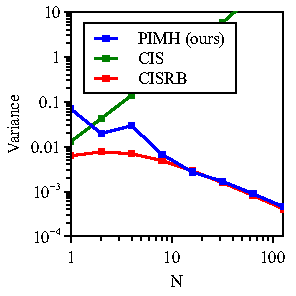
\includegraphics[scale=0.85]{figures/simulations_01.pdf}
  }
  \subfloat[\(\Delta \mu = 2\)]{
    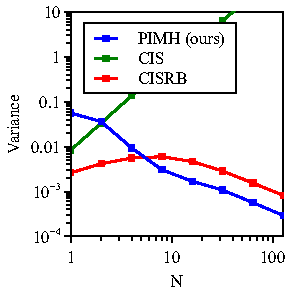
\includegraphics[scale=0.85]{figures/simulations_02.pdf}
  }
  \subfloat[\(\Delta \mu = 4\)]{
    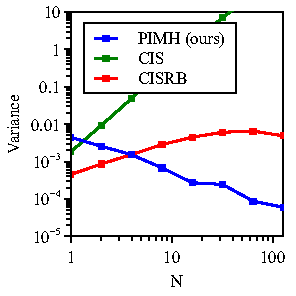
\includegraphics[scale=0.85]{figures/simulations_03.pdf}
  }
  \caption{Conditional variance of different MCMC kernels with varying \(N\) and KL divergence between the proposal and target distribution.
  }\label{fig:simulations}
  \vspace{-0.1in}
\end{figure}

\paragraph{Results Summary}
The results are presented in Figure~\ref{fig:simulations}.
We can see that, when the difference of the mean of the \(p\) and \(q\) is large, the variance of CISRB \textit{increases} with \(N\).
This increasing period becomes longer as the KL divergence between \(p\) and \(q\) increases.
Also, notice that CISRB has much smaller variance compared to CIS due to the Rao-Blackwellization gain.
This effect becomes larger as \(N\) increases.
Unfortunately, however, our experiments did not reveal such great of a performance gain on real-world problems.
PIMH has slightly larger variance compared to \(CIS\) in the small \(N\) regime.
This is due to the higher acceptance rate of the Metropolis-Hastings acceptance ratio compared to Barker's acceptance ratio used by CIS~\citep{peskun_optimum_1973, minh_understanding_2015}.
